\documentclass[12pt, a4paper]{ctexart} % 直接使用中文文档类

% ---------- 页面设置 ----------
\usepackage{algorithm}      % 算法环境
\usepackage{algorithmic}    % 算法伪代码
\usepackage{amsmath, amssymb}   % 数学公式支持
\usepackage{geometry}
\usepackage{indentfirst}   % 让首段也缩进
\usepackage{graphicx}
\usepackage{amsfonts} % 或者使用 \usepackage{amssymb}////为了使用黑体字公式
\usepackage{booktabs}%三线表格式
\usepackage{float}  %固定图片

\setlength{\parindent}{2em} % 缩进2字符(1em≈1汉字宽度)
\geometry{left=3cm, right=2.5cm, top=2.5cm, bottom=2.5cm}

% ---------- 字体配置 ----------
\setmainfont{Times New Roman}          % 设置西文字体

% ---------- 段落格式 ----------
\linespread{1.5}                      % 1.5倍行距
\setlength{\parindent}{2em}           % 首行缩进

% ---------- 标题格式 ----------
\usepackage{titlesec}
\titleformat{\section}{\Large\bfseries\heiti}{\thesection}{1em}{}
\titleformat{\subsection}{\large\bfseries\heiti}{\thesubsection}{1em}{}

% ---------- 文档信息 ----------
\title{IMPACTX:通过适当预测 CorrecT EXplanations 提高模型性能}
\author{译者    Tinkle}
\date{\today}

\begin{document}
\maketitle{}
% ---------- 摘要页 ----------
\begin{abstract}
    可解释的人工智能(XAI)研究主要集中于解释人工智能模型的决策,尤其是深度学习(DL)模型。然而,人们对使用 XAI 技术自动提高人工智能系统本身性能的兴趣也在不断增长。本文提出的 IMPACTX 是一种利用 XAI 作为全自动关注机制的新方法,无需外部知识或人工反馈。实验结果表明,IMPACTX 在模型训练过程中集成了基于 XAI 方法输出的注意力机制,从而提高了独立 ML 模型的性能。此外,IMPACTX 可直接为模型决策提供适当的特征归属图,而无需在推理过程中依赖外部 XAI 方法。我们使用三个广受认可的 DL 模型(EfficientNet-B2、MobileNet 和 LeNet-5)和三个标准图像数据集对我们的建议进行了评估: CIFAR-10、CIFAR-100 和 STL-10。结果表明,在所有评估的数据集上,IMPACTX 始终如一地提高了所有受检 DL 模型的性能,并直接为其响应提供了适当的解释。
    
    关键词 XAI、性能改进、深度学习、解释、归因图
\end{abstract}

% ---------- 正文部分 ----------
\section{介绍}
现代机器学习(ML)和深度学习(DL)方法的内部运作通常是不透明的,这使得人工智能科学家无法解释所提供的输出结果背后的原因。eXplainable Artificial Intelligence(XAI)旨在提供对人工智能模型内部机制和/或其决策背后动机的见解,帮助用户理解 ML 模型产生的结果。XAI 方法已在应用于各类输入的多项人工智能任务中得到采用,包括图像[35, 3, 33]、自然语言处理、临床支持系统[39, 2]等。不过,值得注意的是,虽然现有的 XAI 文献中有相当一部分侧重于为人工智能系统提供解释[26, 31, 8],但 XAI 研究的另一个新目标是改进 ML 系统本身[49]。目前有关这一主题的文献通常介绍需要人类互动的方法,如[46, 40, 18, 36, 32, 56, 42]。在这些作品中,人的作用可被视为一种人工引导注意力的方法,引导模型朝特定的输入特征前进。但最近,人们越来越重视使用 XAI 技术来自主改进机器学习系统,将其作为训练阶段的一部分,而不需要人类的直接干预[49, 43, 27, 44]。

其基本假设是,对模型输出的解释可以改进 ML 系统的训练,从而找到更好的解决方案。特别是,所采用的 XAI 方法可被视为一种注意力机制[48],能够引导模型提高性能(例如,见[16])。这类方法通常涉及改变训练程序或模型的损失函数,以强调相关信息[51, 36, 28]。在本文中,我们介绍了 IMPACTX(通过适当预测 CorrecT eXplanations 提高模型性能),这是一种新颖的方法,它以完全自动化的方式利用人工智能作为一种关注机制,无需外部知识或人工反馈。IMPACTX 实现了两个主要目标: (i) 通过整合在 XAI 方法输出上训练的注意力机制,提高 ML 模型的性能;(ii) 直接为模型的决策提供适当的解释,使整个框架在本质上具有自解释性。值得注意的是,这种自我解释能力是在学习阶段结束时获得的,而在学习阶段,IMPACTX 则依靠外部 XAI 方法来完善和增强模型的自我解释能力。简而言之,这是通过一个双分支模型来实现的:第一个分支由一个特征提取器和一个分类器组成,第二个分支是一个编码器-解码器方案,用于编码分类相关输入特征的有用信息。这两个分支之间的互动可在分类任务期间为分类器提供指导,同时由编码器-解码器分支为给定输出提供解释。正如我们将在第 2 节讨论的那样,IMPACTX 与其他不需要直接人工干预的方法不同,因为 IMPACTX 同时使用了增强的中间特征和增强的损失函数,而且是一种与模型无关的方法。为了评估我们的建议,我们通过实验评估了 IMPACTX 提高 ML 模型性能和以归因图的形式提供有意义解释的能力。该实验评估是在三种广受认可的 DL 模型上进行的: EfficientNet-B2、MobileNet 和 LeNet-5。所有实验均使用三个标准图像数据集进行: CIFAR-10、CIFAR-100 和 STL-10。

本文的组织结构如下:第 2 部分概述了使用 XAI 增强机器学习系统的相关工作。第 3 节详细介绍了我们提出的方法,第 4 节概述了实验评估。第 5 节介绍了实验评估的结果,第 5.3 节对这些结果进行了全面讨论,第 6 节为结束语。

\section{相关工作}
为解决可解释性问题,人们提出了不同类型的解释[9, 14, 35, 29, 41],这取决于所解释的人工智能系统和所采用的 XAI 方法。一种非常常见的方法是根据输入特征的重要性得分(即归因图或相关性图)提供基于视觉的解释。这种方法的例子包括激活最大化(AM)[15]、层相关性传播(LRP)[9]、深度泰勒分解[11, 34]、解卷积网络[53]、上卷积网络[52, 14]和 SHAP 方法[29]。

重要的是,在通过 XAI 方法增强 ML 系统的背景下,这些方法可被视为一种利用外部知识的方法,这些外部知识可由人工干预提供,如归因图的注释,或以完全自动化的方式提供,无需人工操作员参与(例如,见[20, 4])。不过,正如在第 1 节中提到的,我们注意到文献的一个重要方面是在 XAI 的背景下通过人工干预改进 ML 模型,这在一些研究中得到了证明[46, 40, 18, 36, 32, 56, 42]。文献[49]最近对使用 XAI 方法改进 ML 系统的研究工作进行了调查,也可以推断出这一方面。此外,[49] 还讨论了从性能、收敛性、鲁棒性和效率等不同维度改进 ML 模型的工作。为利用 XAI 提高 ML 模型性能,[49] 分离出四种主要方法: i) 增强数据,利用解释生成人工样本或改变数据分布,从而深入了解不良行为[46, 40];ii) 增强中间特征,通过解释测量特征重要性,可有效利用这些信息缩放、屏蔽或转换中间特征,从而改进模型[1, 16, 5, 7]; iii) 增强损失,将基于解释的附加正则化项纳入损失训练函数[36, 22, 27]; iv) 增强梯度,在反向传播过程中,也可以通过改变梯度更新来应用解释提供的特征重要性信息[17]。

如第 3 节所述,所提出的 IMPACTX 方法侧重于提高 ML 系统的性能,它与第 2 类 “增强中间特征 ”和第 3 类 “增强损失 ”相关,在学习步骤中无需人类知识的参与。在这种情况下,即在学习步骤中不涉及人类知识的情况下,通过 XAI 方法以自动化方式提高 ML 系统的性能,[10] 提出了 “引导放大”(Guided Zoom)来提高模型在视觉数据上的性能,尤其是在细粒度分类任务上(即类与类之间存在细微差别的任务)。(IDEAL)在医学图像分析中使用局部解释来选择信息量最大的样本。Guided Zoom [10] 和 IDEAL [30] 方法与我们的方法不同,它们使用 XAI 来增强数据。此外,一些方法[38, 55, 22, 5]使用 XAI 技术屏蔽输入特征,以提高性能。

在 [44] LRP 解释中 [33] 导致 ML 模型专注于小样本分类任务训练阶段的重要特征。文献[27]将两个不同类别的热图对比作为损失函数的一部分。文献[43]提出了一种再训练策略,利用 Shapley 值[29]为分类错误的数据样本分配特定的训练权重,从而改进模型预测。我们要强调的是,前面介绍的所有方法都与我们的建议不同,因为我们同时使用了增强的中间特征和增强的损失函数。

我们要强调的是,前面介绍的所有方法都与我们的建议不同,因为我们同时使用了增强的中间特征和增强的损失函数。

相比之下,[16, 7] 中描述的工作似乎与我们的建议有许多共同之处。特别是,[16] 与我们的建议类似,使用了一个额外的注意力分支,即注意力分支网络 (ABN),来改进深度卷积神经网络 (CNN)。ABN 扩展了类激活映射(CAM)[54],以生成解释并利用这些知识提高性能。然而,ABN 与我们的建议不同,因为它不是一种与模型无关的方法(即它需要访问 ML 模型的内部机制,并且专门用于 CNN 模型),而我们的方法可以应用于任何类型的 ML 模型,而无需了解模型本身的内部机制。此外,ABN 采用基于输入掩码的策略,在训练阶段生成注意力掩码,而我们的方法则利用 XAI 解释增强中间特征和损失训练函数。同样,在 [7] 中,我们提出了一种由额外注意力分支组成的架构,该分支是一个解释编码器,旨在通过 Shapley 值获得的加权平均解释 (WAE) 来增强中间特征[29]。总之,由于 ABN [16] 和 WAE [7] 似乎与我们的提议更为相似,因此我们将在第 5 章中对 ABN、WAE 和本文的提议进行直接比较。5.

\section{IMPACTX 框架}
\subsection{采用的假设和符号}
在最简单的形式下,一个典型的机器学习分类系统 \( \mathcal{A} \) 通常可以被视为由两个主要组件组成:
\begin{itemize}
    \item 特征提取器 \( M \)(例如,在前馈深度神经网络(DNN)模型中,它通常对应于 DNN 的前几层)。
    \item 分类组件 \( Q \)(通常对应于前馈模型中分类过程的剩余部分)。
\end{itemize}
因此,我们有:
\[
\hat{y} = \mathcal{A}(\mathbf{x}) = Q(M(\mathbf{x}))
\]
其中,\( \hat{y} \) 是输入 \( \mathbf{x} \in \mathbb{R}^{d} \) 的估计类别,且 \( Q(M(\mathbf{x})) \in \{1, \dots, K\} \)。

为了不失一般性,在本文中,我们将 \( Q \) 仅视为一个最终的函数,该函数从 \( K \) 个分数向量中计算推测的类别,即:
\[
Q(\mathbf{m}) = \arg\max (\text{softmax}(\mathbf{m}))
\]
其中 \( \mathbf{m} \in \mathbb{R}^{K} \)。在合适的学习过程中,\( M \) 是一个能够将输入 \( \mathbf{x} \) 映射到 \( K \) 维表示空间的模型,其中:
 其第 \( k \) 个分量(\( 1 \leq k \leq K \))表示输入 \( \mathbf{x} \) 属于第 \( k \) 类的分数。

一个典型的 \( M \) 的示例是 DNN 在最终 softmax 层之前的所有层。然而,在一般情况下,任何能够将 \( \mathbf{x} \) 投影到某个特征空间的模型都可以被作为 \( M \)(例如,一系列 DNN 层提取输入 \( \mathbf{x} \) 的特征)。

我们定义 \( y \in \{1, \dots, K\} \) 作为输入 \( \mathbf{x} \) 在 \( K \) 类分类问题中的正确标签。

设:
- \textbf{训练数据集}\( S^T \) 包含 \( N \) 个带标签的样本:
  \[
  S^T = \{ (\mathbf{x}^{(i)}, y^{(i)}) \}_{i=1}^{N}
  \]
- \textbf{测试数据集}\( S^E \) 由 \( J \) 个仅用于评估机器学习模型的样本组成:
  \[
  S^E = \{ (\mathbf{x}^{(j)}, y^{(j)}) \}_{j=1}^{J}
  \]
\subsection{一般描述}
IMPACTX 是一种双分支(double-branch)架构,当应用于分类器 \( \mathcal{A} \) 时,该架构的性能优于独立训练的标准分类器:
\[
\mathcal{A}(\mathbf{x}) = Q(M(\mathbf{x}))
\]
此外,该增强架构还能够提供与输出相关的输入归因图(input attribution maps)。

IMPACTX 框架由两个相互作用的分支组成(参见图 1):

1. \textbf{第一分支(顶部)} 由特征提取器 \( M \) 组成,其能够从输入数据中提取重要特征,以便对输入 \( \mathbf{x} \) 进行分类。此外,该分支还包含一个 \( K \) 类分类器 \( C \),用于返回输入 \( \mathbf{x} \) 的估计类别 \( \hat{y} \)。

2. \textbf{第二分支(底部)} 负责 IMPACTX 的\textbf{注意力机制(attention mechanism)}。它由 潜在解释预测器(Latent Explanation Predictor, LEP)组成,该模块能够从输入特征中提取关键信息,以计算相对于分类响应的输入归因图。此外,该分支还包含一个解码器(Decoder, D),能够有效生成输入 \( \mathbf{x} \) 的归因图。

因此,IMPACTX 的目标是通过利用 \( m = M(\mathbf{x}) \) 和 \( \mathbf{z} = LEP(\mathbf{x}) \) 的输出来建立估计类别:
\[
\hat{y} = C(m, \mathbf{z})
\]
并同时获得相对于 \( \hat{y} \) 的预测归因图 \( \hat{r} \)。

在接下来的章节中,我们将详细讨论 IMPACTX 如何进行训练,以实现该目标。

\subsection{训练 IMPACTX}
IMPACTX 方法的训练阶段如图 1 所示。M 和 LEP 都接收 $x$ 作为输入,产生相应的输出 $m$ 和 $z$。这些输出被连接起来并转发到分类器 C。此外,

\begin{figure}[H]
    \centering
    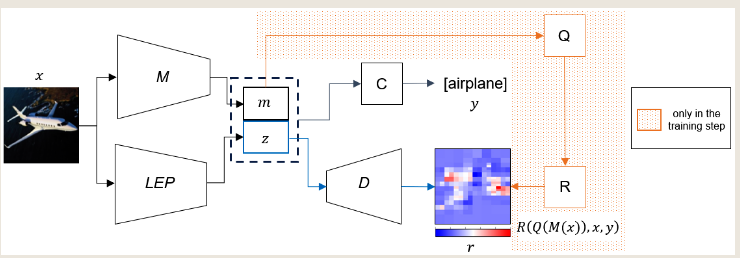
\includegraphics[width=0.9\textwidth]{img/IMPACTX_1.png}
    \caption{ IMPACTX 框架概述。在 IMPACTX 的训练阶段,特征提取器 \( M \) 和潜在解释预测器 \( LEP \) 都接收输入 \( \mathbf{x} \),分别生成 \( \mathbf{m} \) 和 \( \mathbf{z} \)。然后,这些表示被分类器 \( C \) 组合用于分类。特别地,\( LEP \) 和解码器 \( D \) 利用解释函数 \( R(\mathcal{A}(\mathbf{x})), \mathbf{x}, y) \) 来生成可解释性信息。该架构采用融合均方误差(MSE) 和交叉熵(CE) 的损失函数进行训练,以优化解释重建并提高分类性能。在 IMPACTX 的推理阶段,分类器 \( C(\mathbf{m}, \mathbf{z}) \) 预测类别 \( \hat{y} \),而 \( LEP - D(\mathbf{x}) \) 负责重建输入 \( \mathbf{x} \) 的解释 \( r \)。}
\end{figure}


变量 \( \mathbf{z} \) 由解码器 \( D \) 解码,该解码器负责重建解释 \( \mathbf{r} \)。换句话说,\( LEP \) 和 \( D \) 组成一个编码-解码(Encoder-Decoder)结构,其中内部变量 \( \mathbf{z} \) 被用于学习解释的编码。分类器 \( C \) 利用 \( M \) 和 \( LEP \) 的组合知识进行推理。因此,对于一个新的数据点 \( \mathbf{x}^{(j)} \),其估计输出 \( \hat{y}^{(j)} \) 定义为:
\[
\hat{y}^{(j)} = \arg\max \left( \text{softmax} \left( C\left(M(\mathbf{x}^{(j)}), LEP(\mathbf{x}^{(j)})\right) \right) \right).
\]

因此,IMPACTX 旨在同时完成分类任务,并利用解码器 \( D \) 和解释模块 \( LEP \) 构建预测归因图 \( \mathbf{r} \)。

IMPACTX 的有效训练可以通过至少两种方式进行:

\textit{单阶段训练(Single-stage training)}:
所有 IMPACTX 模块同时在训练集 \( S^T \) 上训练,并在每次训练迭代结束时为每个样本 \( \mathbf{r}^{(i)} \) 生成归因图。在这种情况下,使用不断改进的归因图 \( \mathbf{r}^{(i)} \) 可以提高分类性能。理想情况下,这将创建一个正反馈循环,使分类和归因图的生成相互促进。然而,在每次迭代计算归因图可能会消耗大量计算资源,并且由于 \( M \)、\( LEP \) 和 \( D \) 的权重在初始阶段是随机初始化的,生成的归因图 \( \mathbf{r}^{(i)} \) 在早期训练阶段可能缺乏实际意义。

\textit{双阶段训练(Two-stage training)}:
该训练方法分为两个阶段。在第一阶段,整个分类器 \( \mathcal{A}(\cdot) \) 的参数被训练,并在训练集 \( S^T \) 上进行初步评估。在第一阶段结束时,为 \( S^T \) 中的每个样本生成归因图 \( \mathbf{r}^{(i)} \) 并与真实类别标签对应。在第二阶段,剩余模块 \( C \)、\( D \) 和 \( LEP \) 被训练,而 \( M \) 的权重保持不变。特别地,分支 \( LEP-D \) 的目标是重建在第一阶段末计算出的归因图。由于归因图只计算一次,双阶段训练相比于单阶段训练计算成本更低。

无论采用哪种训练方式,该架构的损失函数都结合了均方误差(MSE)和交叉熵(CE):
- 均方误差(MSE)用于度量真实归因图 \( \mathbf{r}^{(i)} \) 与 \( LEP-D \) 分支输出之间的误差。
- 交叉熵(CE)用于度量真实类别标签 \( y^{(i)} \) 与分类器 \( C \) 预测值之间的误差。

损失函数定义如下:
\[
L = CE\left(y^{(i)}, C(m^{(i)}, z^{(i)})\right) + \lambda \cdot MSE\left(r^{(i)}, LEP - D(\mathbf{x}^{(i)})\right)
\]

其中,\( \lambda \) 表示正则化参数。该方法使 \( \mathbf{z}^{(i)} \) 在归因图重建误差的约束下进行优化,同时保持分类性能的稳定性。

\subsection{生成基于归因的解释}
我们使用 XAI 归因方法 \( R \) 生成输入 \( \mathbf{x} \) 的归因图 \( \mathbf{r} \),以描述其关于真实类别标签 \( y \) 在模型 \( \mathcal{A}(\mathbf{x}) \) 下的决策依据。具体而言,对于每个可用的训练数据 \( \mathbf{x}^{(i)} \in S^T \),采用方法 \( R \) 计算其对应于真实类别标签 \( y^{(i)} \) 的归因图 \( \mathbf{r}^{(i)} \),其中:
\[
\mathcal{A}(\mathbf{x}^{(i)}) = Q(M(\mathbf{x}^{(i)}))
\]
目标是获得与训练数据真实类别标签 \( y^{(i)} \) 对齐的归因图 \( \mathbf{r}^{(i)} \)。

因此,我们选择 \( R \) 作为一种 XAI 方法,该方法不仅提供对预测类别的解释,还能针对所有可能的类别进行解释。我们将其表示为:
\[
R(\mathcal{A}, \mathbf{x}, k) = \mathbf{r}_k
\]
其中,\( k \) 表示所需解释的类别。

最终,归因图与训练数据提供的真实类别标签对应,计算结果为:
\[
\mathbf{r}^{(i)} = R(\mathcal{A}(\mathbf{x}^{(i)}), \mathbf{x}^{(i)}, y^{(i)}).
\]
\section{实验装置}
在本节中,我们将介绍一系列实验,旨在评估 IMPACTX 框架的两种不同功能:提高 ML 模型的性能和以归因图的形式提供有意义的解释。我们在几个标准分类任务上对 IMPACTX 的性能进行了评估,并将其结果与文献中的类似方法(即 ABN [16] 和 WAE [7])进行了比较,同时也与 IMPACTX 本身(我们将其视为基线)和底层分支提供的关注机制进行了比较。随后,我们进行了定性和定量分析,以评估 IMPACTX 生成的归因图的有效性。归因图的定性分析侧重于解释如何突出待分类元素的重要部分,我们希望这与人类用户的期望相一致,从而为模型的决策过程提供直观的见解。同时,定量评估采用 MoRF(最相关优先)[37] 曲线来衡量归因图所确定的特征的相关性,从而确定所提供的归因图是否可被视为对框架的可靠解释。以下各小节详细介绍了所使用的数据集、归因生成算法 R、IMPACTX 模块架构和学习程序。

\subsection{数据}
本研究使用的基准数据集包括 CIFAR-10、CIFAR-100 和 STL-10。

\begin{itemize}
    \item \textbf{CIFAR-10}  包含 60,000 张彩色图像,共分为 10 个类别:飞机(airplane)、汽车(automobile)、鸟(bird)、猫(cat)、鹿(deer)、狗(dog)、青蛙(frog)、马(horse)、船(ship)和卡车(truck)。数据集分为 50,000 张训练图像和 10,000 张测试图像,每张图像的尺寸为 \( 32 \times 32 \) 像素。

    \item \textbf{CIFAR-100} 包含 60,000 张彩色图像,共分为 100 个类别,其中 50,000 张用于训练,10,000 张用于测试。所有图像的尺寸均为 \( 32 \times 32 \) 像素。

    \item \textbf{STL-10} 数据集包含 10 个类别的图像,类别分别为:飞机(airplane)、鸟(bird)、汽车(car)、猫(cat)、鹿(deer)、狗(dog)、马(horse)、猴子(monkey)、船(ship)和卡车(truck)。每张图像的尺寸为 \( 96 \times 96 \) 像素。数据集包括 5,000 张训练图像和 8,000 张测试图像。
\end{itemize}
\subsection{解释生成器算法}
我们采用了 SHAP 方法 [29] 作为 R。之所以选择这个项目,是因为 SHAP 是 XAI 中一项重要的技术,它根据属性映射提供解释,并且不仅为预测的类提供解释,还根据我们的方法的要求为每个可能的类提供解释。特别是在这项研究中,我们采用了 Partition Explainer 算法作为 SHAP 的特定版本,进行了 2000 次评估以获得最终解释 [29]。
\subsection{IMPACTX 模块和两阶段培训}
我们使用三种不同的 M 模型对 IMPACTX 进行了评估:LeNet-5 [25]、在 ImageNet [13] 上预先训练的 MobileNet [19],以及在噪声学生权重 [50] 上预先训练的 EfficientNet-B2 [45]。本研究的重点在于解释模型和说明输入特征对模型预测的影响。Latent Explanation Predictor LEP 模块从选定的 A 结构开始构建,用一个维度为 512 的全连接层和一个 sigmoid 激活函数取代了最后一个全连接层。用于 CIFAR-10 和 CIFAR-100 数据集的解码器结构如图 2 所示。对于 STL-10,由于 STL-10 图像的输入维度与 CIFAR-10/100 不同,解码器中包含了额外的[Conv、Conv、UpSampling]层序列。需要再次强调的是,潜在解释预测器-解码器(LEP-D)提取的是与输入图像的视觉特征和训练阶段发现的相应归因分数相关的洞察力和关系。M 和 LEP 的输出分别代表从 x 提取的特征和编码归因 z,它们被连接起来,然后输入最终分类器 C。

\begin{table}[h]
  \centering
  \caption{网格搜索优化策略的变化范围}
  \label{tab:grid_search}
  \begin{tabular}{|l|l|}
      \hline
      \textbf{Hyperparameter} & \textbf{Range} \\ \hline
      Batch Size & \{16, 32, 64\} \\ \hline
      \(\mathcal{A}\) Learning Rate & [0.0001, 0.01] with step of 0.0005 \\ \hline
      Validation Fraction & \{0.05, 0.1, 0.2\} \\ \hline
      \textit{IMPACTX} \(\lambda\) & [0.2, 1.4] with step of 0.2 \\ \hline
  \end{tabular}
\end{table}

正如第 3.3 节所讨论的,我们采用了双阶段训练(two-stage training),因为它比单阶段训练(single-stage training)计算成本更低。因此,在第一阶段学习中,通过网格搜索(grid-search)方法确定超参数批量大小(batch size)、学习率(learning rate)和验证比例(validation fraction),并在所选数据集上微调每个 \( \mathcal{A} \) 模型。网格搜索的范围详见表 1。
在第一阶段学习完成后,在第二阶段学习中,训练 \( LEP \)、\( D \) 和 \( C \) 的参数,同时保持 \( M \) 的参数固定(见图 1)。\( D \) 的结构如图 2 所示。正则化参数 \( \lambda \) 的最优值通过超参数网格搜索(grid-search)确定,其搜索范围详见表 1。最终,在测试集上计算每个数据集的最终性能。

\begin{figure}[H]
  \centering
  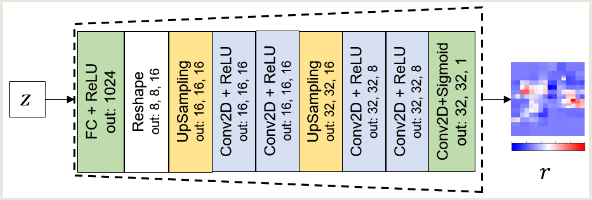
\includegraphics[width=0.9\textwidth]{img/IMPACTX_2.png}
  \caption{为 CIFAR-10 和 CIFAR100 数据集设计的解码器架构。该架构由一个卷积层(Conv2D)、一个全连接层(FC)和一个上采样层组成。所有卷积层的内核大小都是 3 × 3,而过滤器的数量则由输出形状的三个维度决定。}
\end{figure}

\subsection{评价措施}

我们评估了 IMPACTX 在分类任务中的性能,以及它生成的归因图(attribution maps)。分类任务的性能通过标准测试集上的准确率进行衡量。所提出的方法与基线模型 \( \mathcal{A} \) 进行了比较分析(其中 \( \mathcal{A} \) 可以看作是 IMPACTX 本身,但不包括由底部分支提供的注意力机制),以及 ABN 和 WAE 方法。

归因图的评估采用定性和定量两种方式,分别报告所获得的归因图示例和 MoRF(Most Relevant First)曲线。MoRF 曲线广泛应用于 XAI 研究中,以评估所提出的解释 。本质上,图像区域按照归因图所指示的相关性值的降序顺序,被迭代地用随机噪声替换,并输入到机器学习模型中。因此,归因图中标记的特征对分类输出越重要,则曲线的陡峭程度越大。

MoRF 曲线提供了一种定量评估方式,以衡量归因图对机器学习系统行为的解释程度。同时,定性分析有助于理解所得解释与用户的直觉预期的匹配程度,而定量分析则用于衡量归因图作为解释的有效性。

\section{结果与讨论}

\subsection{性能}

表 \ref{tab:accuracy_results} 显示了不同架构 \( \mathcal{A}(\cdot) \)(包括 LeNet-5、MobileNet 和 EfficientNet-B2)在 CIFAR-10、CIFAR-100 和 STL-10 测试集上的性能。该表报告了 IMPACTX 方法(IMPACTX 列)和基线模型(Baseline 列)在分类准确率方面的对比结果。此外,还列出了 ABN  和 WAE方法的结果。

\begin{table}[h]
    \centering
    \caption{CIFAR-10、CIFAR-100 和 STL-10 测试集上的准确率(\%)。最佳结果以 \textbf{粗体} 显示。}
    \label{tab:accuracy_results}
    \begin{tabular}{l|c|c|c|c}
        \hline
        \textbf{Model} & \textbf{Baseline \( \mathcal{A} \)} & \textbf{IMPACTX} & \textbf{ABN } & \textbf{WAE } \\ 
        \hline
        \multicolumn{5}{c}{\textbf{CIFAR-10}} \\ 
        \hline
        LeNet-5 & 67.96 & \textbf{70.65} & 68.49 & 68.10 \\ 
        MobileNet & 94.63 & \textbf{96.27} & 95.41 & 94.75 \\ 
        EfficientNet-B2 & 98.06 & \textbf{98.38} & 98.19 & 98.08 \\ 
        \hline
        \multicolumn{5}{c}{\textbf{CIFAR-100}} \\ 
        \hline
        LeNet-5 & 36.23 & \textbf{39.49} & 37.62 & 36.20 \\ 
        MobileNet & 76.72 & \textbf{79.37} & 78.24 & 76.98 \\ 
        EfficientNet-B2 & 87.88 & \textbf{89.06} & 88.89 & 88.27 \\ 
        \hline
        \multicolumn{5}{c}{\textbf{STL-10}} \\ 
        \hline
        LeNet-5 & 52.59 & \textbf{55.86} & 53.36 & 52.99 \\ 
        MobileNet & 91.07 & \textbf{95.79} & 92.71 & 91.42 \\ 
        EfficientNet-B2 & 98.76 & \textbf{99.00} & 98.59 & 98.65 \\ 
        \hline
    \end{tabular}
\end{table}

IMPACTX 在所有所选数据集上均相较于基线模型实现了均匀的提升,并且该提升与所使用的分类架构无关。此外,与其他选定方法相比,IMPACTX 也取得了更好的结果。
\begin{figure}[H]
  \centering
  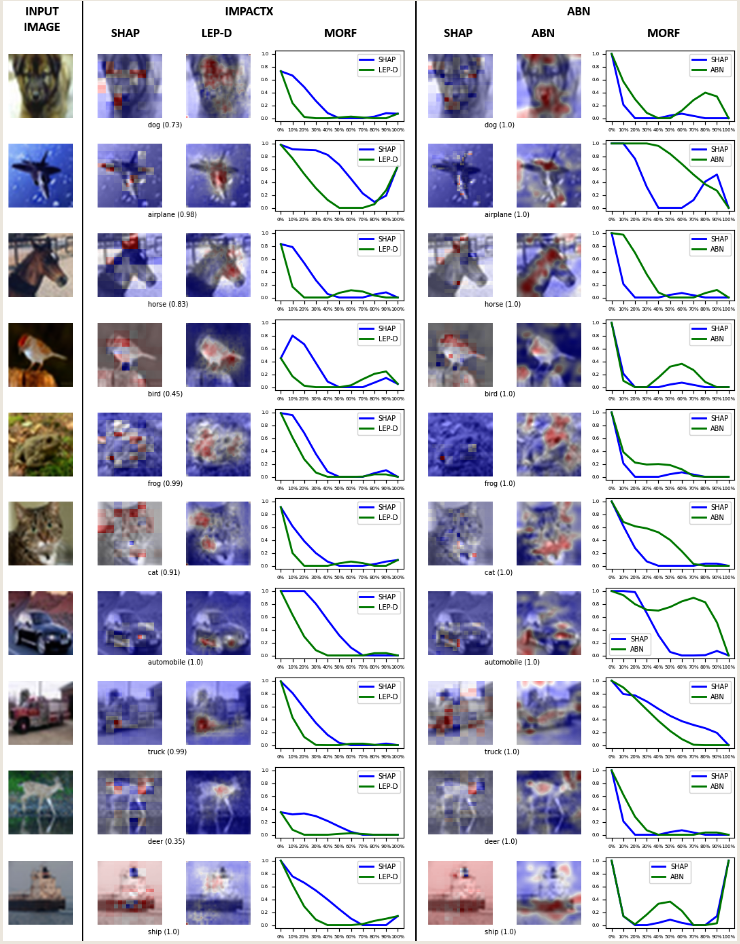
\includegraphics[width=0.9\textwidth]{img/IMPACTX_3.png}
  \caption{来自 CIFAR-10 测试集的图像。图像已经过过滤,以实现更好的可视化效果。}
\end{figure}

\begin{figure}[H]
  \centering
  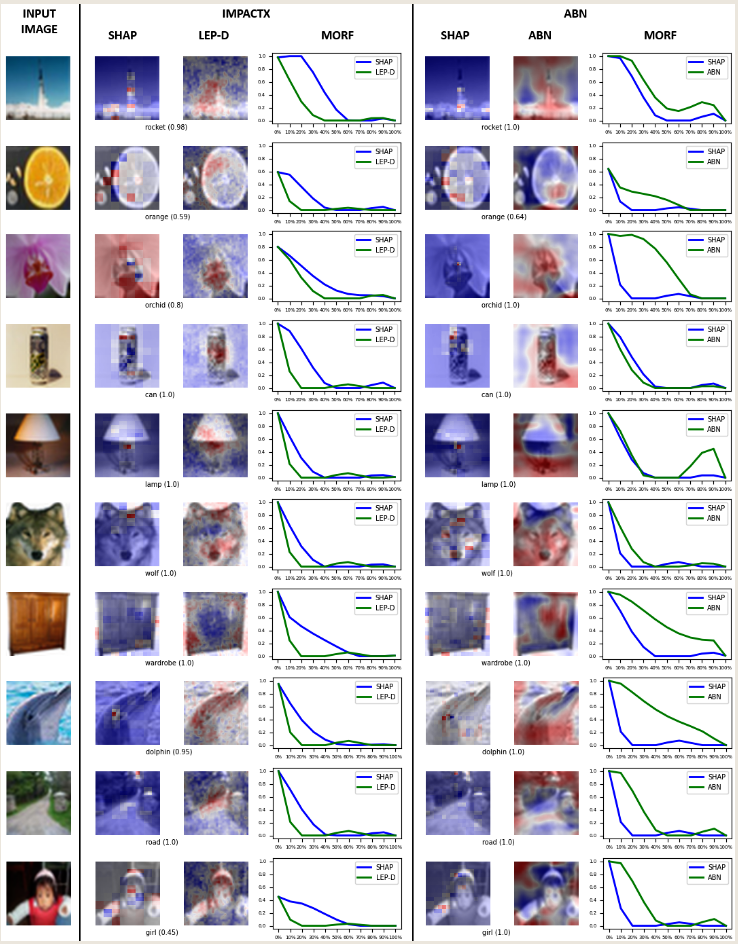
\includegraphics[width=0.9\textwidth]{img/IMPACTX_4.png}
  \caption{来自 CIFAR-100 测试集的图像。图像已经过过滤,以实现更好的可视化效果。}
\end{figure}


\subsection{评估归因映射}

在本节中,我们希望评估由 IMPACTX 直接生成的归因图是否可以被视为 IMPACTX 分类响应的解释。为此,我们将它们与其他方法提供的解释进行比较。
\begin{figure}[H]
  \centering
  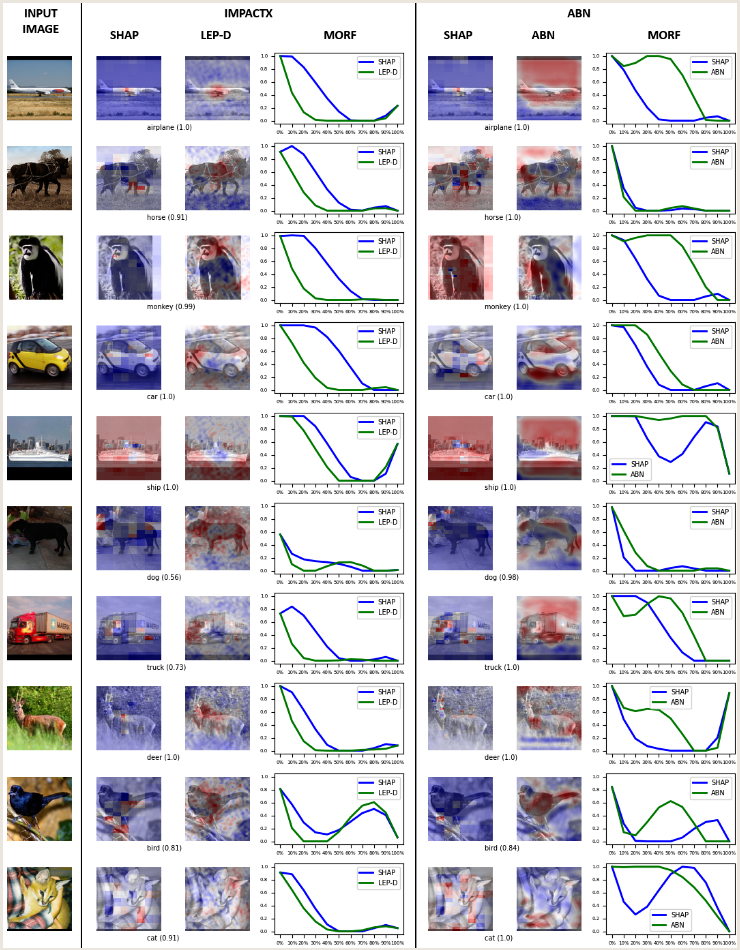
\includegraphics[width=0.9\textwidth]{img/IMPACTX_5.png}
  \caption{来自 STL-10 测试集的图像。图像已经过过滤,以实现更好的可视化效果。}
\end{figure}
具体来说,我们提供了 IMPACTX 预测的类别及其对应的置信度分数。此外,在相同的图示中,报告了由解释方法 SHAP 生成的归因图(第 2 列),以及 IMPACTX 生成的归因图(第 3 列)。对于每个输入,还报告了 SHAP 和 IMPACTX 归因图的 MoRF(Most Relevant First)曲线(第 4 列)。相同的比较也针对 ABN 体系结构进行了分析(右侧)。

有趣的是,IMPACTX 和 ABN 在定性上都强调了与各自类别直观相关的输入特征。然而,MoRF 曲线在定量上揭示了不同的行为。具体而言,MoRF 曲线表明,与 SHAP 选择的特征相比,ABN 识别出的最相关特征对分类的影响较小。相反,在 IMPACTX 和 SHAP 之间观察到了相反的模式。IMPACTX 突出的最相关特征比 SHAP 识别的特征对分类更具影响力。

\subsection{讨论}
实验结果表明,与未使用 IMPACTX 框架的 ML 模型相比,IMPACTX 在分类任务中的表现更好,同时提供的归因图可被视为比事后 XAI 方法提供的归因图更可靠的解释。特别是在性能方面,IMPACTX 分支之间的互动增强了模型关注相关特征的能力,从而提高了分类性能。在训练过程中,IMPACTX 会强调与模型决策相关的特征,从而获得更准确的结果。事实上,IMPACTX 的训练过程就是为了将重点放在对模型决策具有重要意义的特征上。此外,关于底层分支构建归因图的问题,IMPACTX 能够提供准确的归因图可归功于其在推理时将决策和论证整合在一起的方法,这与 SHAP 等事后方法的外部性形成了鲜明对比。这种整合使 IMPACTX 能够生成更准确反映模型决策过程的归因图。有趣的是,与 ABN 相比,IMPACTX 生成的归因图似乎具有更好的解释性。这很可能是因为 IMPACTX 的注意机制旨在考虑训练过程中的真实类别标签,而 ABN 基于 CAM 的方法则依赖于训练过程中获得的类别分数。

\section{结论}
总之,实验结果表明,IMPACTX 能够将 XAI 策略纳入 ML 管道,而不会影响性能。此外,IMPACTX 还能在推理时为其输出计算有效解释,而无需在推理过程后依赖外部 XAI 方法。特别是,实验评估显示了内置的潜在解释预测器 LEP 在提取有用知识方面的有效性。这些知识既可用于 ML 任务,也可用于提供有关模型输出的解释。值得注意的是,LEP 是基于特定 XAI 方法从模型训练集中提取的与真实类别相关的解释构建的,而解码器 D 则能够提供与模型输出相关的有用解释。在未来的研究中,采用不同于用于训练 IMPACTX 框架的 XAI 方法、架构和数据集来探索这种方法的影响可能会很有价值。此外,在本研究中,IMPACTX 是使用第 3.3 节所述的两阶段训练方法进行训练的。3.3 中所述的两阶段训练方法进行训练,而这一选择主要是受计算资源限制所驱动。因此,在未来的工作中,比较两阶段训练和单阶段训练可能会很有意义。最后,我们注意到,对 IMPACTX 归因图的定性分析似乎表明,ML 系统及其在解释 MoRF 曲线所证实的模型决策方面的可靠性,倾向于关注与人类在决策时可能关注的方面相似的方面。虽然这一方面的问题需要在今后的工作中进行更好的研究,但这种可能的一致性表明,模型已经有效地学会了优先考虑与任务内在相关的特征,这与人类处理相同任务的方式类似。值得注意的是,这种类似人类的关注点似乎不仅增强了模型决策的可解释性,还有助于提高执行 ML 任务的性能,如第 5 章所示。








\end{document}
